% ----------------------------------------------------------------- %
%             The Speech Signal Processing Toolkit (SPTK)           %
%             developed by SPTK Working Group                       %
%             http://sp-tk.sourceforge.net/                         %
% ----------------------------------------------------------------- %
%                                                                   %
%  Copyright (c) 1984-2007  Tokyo Institute of Technology           %
%                           Interdisciplinary Graduate School of    %
%                           Science and Engineering                 %
%                                                                   %
%                1996-2011  Nagoya Institute of Technology          %
%                           Department of Computer Science          %
%                                                                   %
% All rights reserved.                                              %
%                                                                   %
% Redistribution and use in source and binary forms, with or        %
% without modification, are permitted provided that the following   %
% conditions are met:                                               %
%                                                                   %
% - Redistributions of source code must retain the above copyright  %
%   notice, this list of conditions and the following disclaimer.   %
% - Redistributions in binary form must reproduce the above         %
%   copyright notice, this list of conditions and the following     %
%   disclaimer in the documentation and/or other materials provided %
%   with the distribution.                                          %
% - Neither the name of the SPTK working group nor the names of its %
%   contributors may be used to endorse or promote products derived %
%   from this software without specific prior written permission.   %
%                                                                   %
% THIS SOFTWARE IS PROVIDED BY THE COPYRIGHT HOLDERS AND            %
% CONTRIBUTORS "AS IS" AND ANY EXPRESS OR IMPLIED WARRANTIES,       %
% INCLUDING, BUT NOT LIMITED TO, THE IMPLIED WARRANTIES OF          %
% MERCHANTABILITY AND FITNESS FOR A PARTICULAR PURPOSE ARE          %
% DISCLAIMED. IN NO EVENT SHALL THE COPYRIGHT OWNER OR CONTRIBUTORS %
% BE LIABLE FOR ANY DIRECT, INDIRECT, INCIDENTAL, SPECIAL,          %
% EXEMPLARY, OR CONSEQUENTIAL DAMAGES (INCLUDING, BUT NOT LIMITED   %
% TO, PROCUREMENT OF SUBSTITUTE GOODS OR SERVICES; LOSS OF USE,     %
% DATA, OR PROFITS; OR BUSINESS INTERRUPTION) HOWEVER CAUSED AND ON %
% ANY THEORY OF LIABILITY, WHETHER IN CONTRACT, STRICT LIABILITY,   %
% OR TORT (INCLUDING NEGLIGENCE OR OTHERWISE) ARISING IN ANY WAY    %
% OUT OF THE USE OF THIS SOFTWARE, EVEN IF ADVISED OF THE           %
% POSSIBILITY OF SUCH DAMAGE.                                       %
% ----------------------------------------------------------------- %
\hypertarget{df2}{}
\name{df2}{second order standard form digital filter}{digital filter}

\begin{synopsis}
 \item[df2] [ --f $f_0$ ] [ --p $f_1 \; b_1$ ] [ --z $f_2 \; b_2$ ] 
            [ {\em infile} ]
\end{synopsis}

\begin{qsection}{DESCRIPTION}
{\em df2} filters data from {\em infile} (or standard output) 
using a second order digital filter in standard form, 
sending the result to standard output.
The central frequency and frequency band can
  be both assigned through the options, shown bellow.
  The filter transfer function is given by:
  \begin{displaymath}
   H(z)=\frac{1-2\exp(-\pi b_2/f_0)\cos(2\pi f_2/f_0)z^{-1} +
        \exp(-2\pi b_2/f_0)z^{-2}}
   {1-2\exp(-\pi b_1/f_0)\cos(2\pi f_1/f_0)z^{-1}+\exp(-2\pi b_1/f_0)z^{-2}}
  \end{displaymath}
 Also, if this command is used in cascade, an arbitrary filter can be
 designed by using the options --p and --z.
 Input and output data are in float format.
\end{qsection}

\begin{options}
        \argm{f}{f_0}{sampling frequency $f_0$ [kHz]}{10.0}
        \argm{p}{f_1 \; b_1}{center frequency $f_1$ [Hz]
                and band width $b_1$ [Hz] of pole}{N/A}
        \argm{z}{f_2 \; b_2}{center frequency $f_2$ [Hz]
                and band width $b_2$ [Hz] of zero}{N/A}
\end{options} 

\begin{qsection}{EXAMPLE}
The command below gives the impulse response of a filter with
a pole at 2000 Hz and a frequency band of 200 Hz:
\begin{quote}
 \verb!impulse | df2 -p 2000 200 | fdrw | xgr !
\end{quote}
\hspace{3cm}
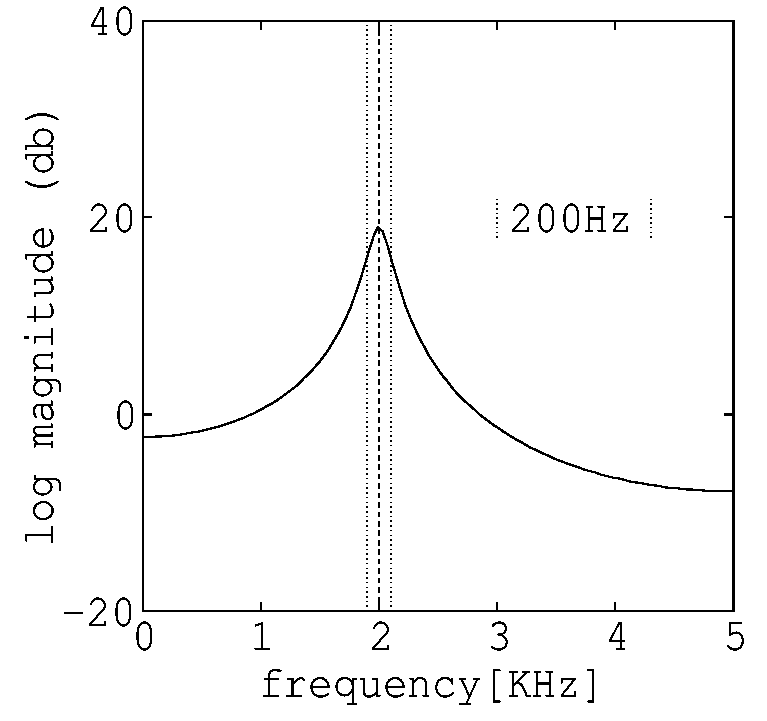
\includegraphics[width=4cm]{fig/df2.eps}
\end{qsection}
